\chapter{Physics of neutrinos beyond the Standard Model}

% --------------------------------------------------------
% ----------------- FLAVOUR OSCILLATIONS -----------------
% --------------------------------------------------------
\section{Flavour oscillations}

% --------------------------------------------------------
% ---------------- EXPERIMENTAL EVIDENCES ----------------
% --------------------------------------------------------
\subsection{Experimental evidence: the solar neutrino problem}
\label{subsec:oscillation-experiments}
\begin{wrapfigure}{l}{0.54\textwidth}
    \centering
    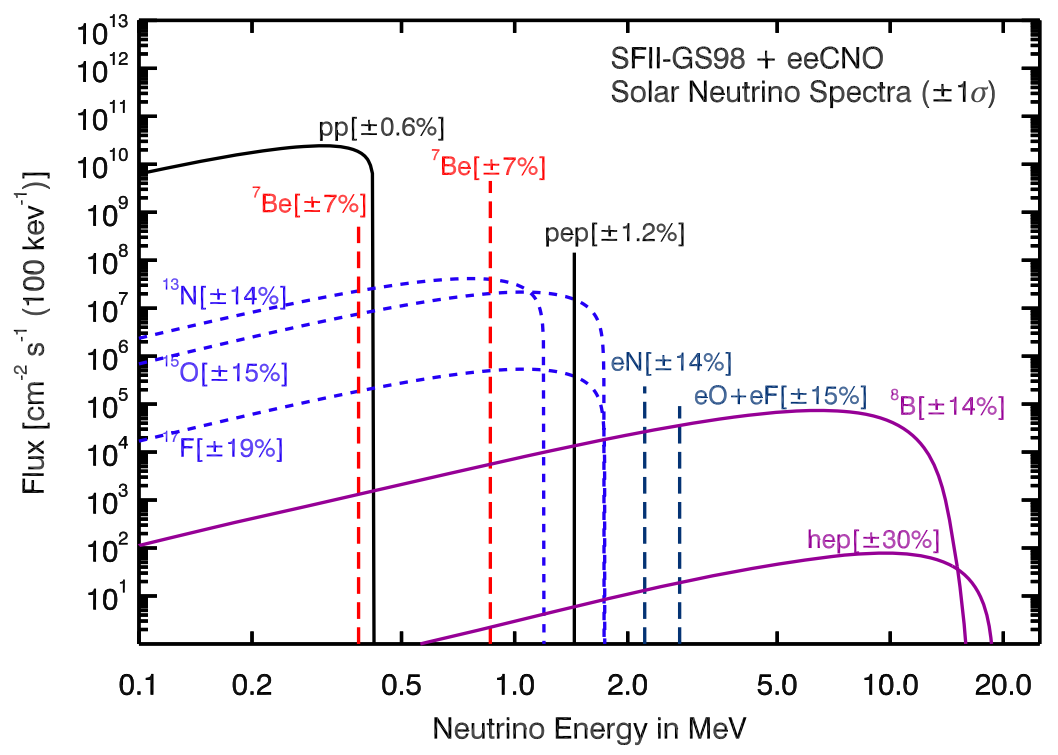
\includegraphics[width=\linewidth]{figures/neutrino-fluxes.png}
    \caption{Energy spectra of solar neutrino fluxes of different reaction processes. Plot taken from \cite{SunNuFluxes}.}
    \label{fig:neutrino-fluxes}
\end{wrapfigure}
As reviewed in \cite{neutrinosPDG}, from which the following discussion is elaborated unless otherwise specified, electron neutrinos are produced in the Sun in thermonuclear reactions that generate solar energy, namely \ac{pp} chains and \ac{CNO} cycles. Based on the \ac{SSM}, the total neutrino flux at Earth can be estimated from the solar luminosity ($L_{\odot} \approx 3.828 \times 10^{26}$~W), dividing it by the net energy released per complete \ac{pp} chain and accounting for the spherical propagation of the neutrinos across the Earth--Sun distance ($1$~AU). In the \ac{pp} chains, which include several neutrino-producing reactions, four protons fuse into a ${}^4$He nucleus, $4p \to {}^4\text{He} + 2e^+ + 2\nu_e$, releasing $Q = 4M({}^1\text{H}) - M({}^4\text{He}) \sim 26.73$~MeV per chain; using atomic masses automatically includes the annihilation of the two positrons with electrons of the plasma. Only a small fraction of this energy, on average $\langle E_{2\nu}\rangle \simeq 0.59$~MeV, is carried away by the two neutrinos, while the rest heats the Sun and is eventually radiated as photons.

In the \ac{CNO} cycles, neutrinos are mainly produced via the decays of ${}^{13}\text{N}$, ${}^{15}\text{O}$ and ${}^{17}\text{F}$. Additionally, electron capture on ${}^{13}\text{N}$, ${}^{15}\text{O}$ and ${}^{17}\text{F}$ produces monoenergetic line spectra of neutrinos, generally referred to as \textit{ecCNO} neutrinos. Compared to the \ac{pp} chains, \ac{CNO} neutrinos carry away a higher fraction of the reaction energy, with average neutrino energies typically ranging between $0.7$~MeV and $1.2$~MeV. However, the flux of \ac{CNO} neutrinos is roughly two orders of magnitude lower than the \ac{pp} one, the \ac{CNO} cycles accounting for less than $1\%$ of the solar energy production, so that they can be neglected in the flux estimate.

Both \ac{pp} reactions and \ac{CNO} ones produce only $\nu_e$: in the absence of oscillations, state-of-the-art calculations predict a \ac{pp} neutrino flux at Earth of approximately $\Phi_\text{pp}(\nu_e) \approx 6 \times 10^{10}~\text{cm}^{-2}\,\text{s}^{-1}$, while the expected fluxes of the individual components are shown in Figure~\ref{fig:neutrino-fluxes}.

\paragraph{The Homestake mine experiment}
Solar neutrinos have been detected since the late 1960s. The first solar neutrino experiment, led by Raymond Davis, was performed underground in the Homestake gold mine in South Dakota, in order to prevent contamination from cosmic-ray induced reactions, which produce ${}^{37}\text{Ar}$ through (p,\,n) processes. It employed liquid tetrachloroethylene (C$_2$Cl$_4$) as the target, exploiting the \ac{CC} interaction $\nu_e + {}^{37}\text{Cl} \longrightarrow e^- + {}^{37}\text{Ar}$, whose threshold of $814$~keV makes it mainly sensitive to ${}^{7}$Be and ${}^{8}$B neutrinos. The produced ${}^{37}\text{Ar}$, with a half-life of $34.8$~days, was chemically extracted every few months and introduced into a low-background proportional chamber, where the Auger electrons emitted in its electron capture were counted to determine the neutrino-${}^{37}\text{Cl}$ reaction rate. The measured rate was less than one third of the expected one, giving rise to the so-called \textit{solar neutrino problem}: the final result was $2.56 \pm 0.16 \pm 0.16 \text{ SNU}$\footnote{SNU (solar neutrino unit) is a unit of event rate defined as $1 \text{ SNU} = 10^{-36}\text{ captures per second per target atom}$. The measured quantity is a capture rate, $R = \sum_i \Phi_i \sigma_i$, summed over the solar neutrino components $i$; converting it into a flux requires assuming the shape of the spectrum.}~\cite{HomestakeResults}, to be compared with the \ac{SSM} prediction of $8.46^{+0.87}_{-0.88} \text{ SNU}$~\cite{SSMReference}.

\paragraph{Gallium-based experiments}
Later, at the turn of the 1990s, two radiochemical experiments were launched: SAGE at the Baksan Neutrino Observatory and GALLEX (later followed by the Gallium Neutrino Observatory, GNO) at the Laboratori Nazionali del Gran Sasso (LNGS). Both exploited the gallium \ac{CC} interaction $\nu_e + {}^{71}\text{Ga} \longrightarrow e^- + {}^{71}\text{Ge}$, whose low threshold of $233$~keV makes it sensitive mainly to \ac{pp} neutrinos, with secondary contributions from ${}^{7}\text{Be}$ ones, i.e. to the lower-energy components of the spectrum of Figure~\ref{fig:neutrino-fluxes}. Following an approach analogous to Homestake, the produced ${}^{71}\text{Ge}$ nuclei, which decay via electron capture with a half-life of $11.4$~days, were chemically extracted to measure the capture rate. SAGE reported $65.4^{+3.1+2.6}_{-3.0-2.8}$ SNU and GALLEX/GNO $69.3 \pm 4.1 \pm 3.6$ SNU, both in sharp contrast with the \ac{SSM} prediction of $127.9^{+8.1}_{-8.2}$ SNU for the same energy range, reinforcing the solar neutrino deficit puzzle.

\paragraph{The Kamiokande experiment}
Starting from the late 1980s, the Kamiokande and Super-Kamiokande water Cherenkov detectors, located in the Kamioka mine in Japan, pioneered real-time measurements of solar neutrino fluxes via \ac{ES} on electrons, written in Eq.~\ref{eq:CC-NCwater} and displayed in Figure~\ref{fig:feynman-CCandNCint}. Kamiokande employed $3000$~t of water, while its successor Super-Kamiokande, running since 1996, contains $50$~kt of ultrapure water.
\begin{equation}
    \label{eq:CC-NCwater}
    \nu_\ell + e^- \longrightarrow \nu_\ell + e^-
\end{equation}
\begin{figure}[H]
    \centering
    \resizebox{0.7\textwidth}{!}{
        % --- Diagramma 1: Corrente Carica (CC) ---
\begin{tikzpicture}[
    thick,
    fermion/.style={draw=black, postaction={decorate},
        decoration={markings, mark=at position 0.55 with {\arrow{latex}}}},
    boson/.style={draw=black, decorate,
        decoration={snake, amplitude=1.5pt, segment length=5pt}},
    dot/.style={circle, fill=black, minimum size=4pt, inner sep=0pt}
]
    \coordinate (V1) at (0, 1.2);
    \coordinate (V2) at (0, -1.2);
    
    \draw[fermion] (-1.5, 1.8) node[left] {$\nu_e$} -- (V1);
    \draw[fermion] (V1) -- (1.5, 1.8) node[right] {$e^-$};
    \draw[fermion] (-1.5, -1.8) node[left] {$e^-$} -- (V2);
    \draw[fermion] (V2) -- (1.5, -1.8) node[right] {$\nu_e$};
    
    \draw[boson] (V1) -- node[right, xshift=2pt] {$W^+$} (V2);
    
    \node[dot] at (V1) {};
    \node[dot] at (V2) {};
\end{tikzpicture}
\hspace{2.5 cm}
% --- Diagramma 2: Corrente Neutra (NC) ---
\begin{tikzpicture}[
    thick,
    fermion/.style={draw=black, postaction={decorate},
        decoration={markings, mark=at position 0.55 with {\arrow{latex}}}},
    boson/.style={draw=black, decorate,
        decoration={snake, amplitude=1.5pt, segment length=5pt}},
    dot/.style={circle, fill=black, minimum size=4pt, inner sep=0pt}
]
    \coordinate (V3) at (0, 1.2);
    \coordinate (V4) at (0, -1.2);
    
    \draw[fermion] (-1.5, 1.8) node[left] {$\nu_\ell$} -- (V3);
    \draw[fermion] (V3) -- (1.5, 1.8) node[right] {$\nu_\ell$};
    \draw[fermion] (-1.5, -1.8) node[left] {$e^-$} -- (V4);
    \draw[fermion] (V4) -- (1.5, -1.8) node[right] {$e^-$};
    
    \draw[boson] (V3) -- node[right, xshift=2pt] {$Z^0$} (V4);
    
    \node[dot] at (V3) {};
    \node[dot] at (V4) {};
\end{tikzpicture}
    }
    \caption{Feynman diagrams of neutrino-electron scatterings. On the left, the \ac{CC} interaction mediated by a $W^+$ boson; on the right, the \ac{NC} 
    interaction mediated by the $Z^0$ boson. The subscript $\ell$ denotes a generic lepton flavour ($\ell = e, \mu, \tau$).}
    \label{fig:feynman-CCandNCint}
\end{figure}
This signal is an indistinguishable mixture of \ac{CC} and \ac{NC} events, dominated by $\nu_e$ thanks to its larger cross-section: being the only flavour that can also interact via the \ac{CC}, $\nu_e$ has a cross-section approximately six times larger than that of $\nu_\mu$ or $\nu_\tau$, so that the detector cannot cleanly measure the total, flavour-independent neutrino flux. Due to energy thresholds of $6.5$~MeV in Kamiokande and $3.5$~MeV in Super-Kamiokande, these experiments are sensitive mainly to ${}^8\text{B}$ neutrinos: Super-Kamiokande measured a flux of $(2.345 \pm 0.014 \pm 0.036) \times 10^{6} \text{ cm}^{-2}\text{s}^{-1}$~\cite{latestSUPERK}. This reveals a severe deficit compared to the theoretical \ac{SSM} prediction for ${}^8\text{B}$ neutrinos of $(5.46 \pm 0.66) \times 10^{6} \text{ cm}^{-2}\text{s}^{-1}$.

\paragraph{Solution to the solar neutrino problem: the SNO experiment}
Finally, the Sudbury Neutrino Observatory (SNO), located in the Creighton Mine near Sudbury (Ontario, Canada) and operated between the late 1990s and the early 2000s, provided the model-independent proof that solar $\nu_e$ change flavour, using $1000$~t of heavy water ($\text{D}_2\text{O}$) contained in a spherical acrylic vessel surrounded by a light-water ($\text{H}_2\text{O}$) shield. Deuterium allowed SNO to observe ${}^8\text{B}$ neutrinos not only through the \ac{ES} channel of Eq.~\ref{eq:CC-NCwater}, as Kamiokande, but also to measure separately the \ac{CC} interaction, sensitive only to $\nu_e$, and the \ac{NC} interaction, which breaks the deuteron apart and is sensitive to all active flavours with equal cross-sections. Both interactions are written in Eq.~\ref{eq:deuteron-interactions} and shown in Figure~\ref{fig:feynman-deuteron}.
\begin{equation}
    \label{eq:deuteron-interactions}
    \begin{aligned}
        \nu_e + d &\longrightarrow e^- + p + p \quad (\text{\ac{CC}})\\
        \nu_\ell + d &\longrightarrow \nu_\ell + p + n \quad (\text{\ac{NC}})
    \end{aligned}
\end{equation}
\begin{figure}[H]
    \centering
    \resizebox{0.7\textwidth}{!}{
        % --- Diagramma 1: Corrente Carica (CC) per SNO ---
\begin{tikzpicture}[
    thick,
    fermion/.style={draw=black, postaction={decorate},
        decoration={markings, mark=at position 0.55 with {\arrow{latex}}}},
    boson/.style={draw=black, decorate,
        decoration={snake, amplitude=1.5pt, segment length=5pt}},
    dot/.style={circle, fill=black, minimum size=4pt, inner sep=0pt}
]
    \coordinate (V1) at (0, 1.2);
    \coordinate (V2) at (0, -1.2);
    
    % Linea superiore: neutrino -> elettrone
    \draw[fermion] (-1.5, 1.8) node[left] {$\nu_e$} -- (V1);
    \draw[fermion] (V1) -- (1.5, 1.8) node[right] {$e^-$};
    
    % Linee inferiori: neutrone che diventa protone, e protone spettatore
    \draw[fermion] (-1.5, -1.8) node[left] {$n$} -- (V2);
    \draw[fermion] (V2) -- (1.5, -1.8) node[right] {$p$};
    \draw[fermion] (-1.5, -2.4) node[left] {$p$} -- (1.5, -2.4) node[right] {$p$};
    
    % Bosone scambiato W+
    \draw[boson] (V1) -- node[right, xshift=2pt] {$W^+$} (V2);
    
    \node[dot] at (V1) {};
    \node[dot] at (V2) {};
\end{tikzpicture}
\hspace{2.5 cm}
% --- Diagramma 2: Corrente Neutra (NC) per SNO ---
\begin{tikzpicture}[
    thick,
    fermion/.style={draw=black, postaction={decorate},
        decoration={markings, mark=at position 0.55 with {\arrow{latex}}}},
    boson/.style={draw=black, decorate,
        decoration={snake, amplitude=1.5pt, segment length=5pt}},
    dot/.style={circle, fill=black, minimum size=4pt, inner sep=0pt}
]
    \coordinate (V3) at (0, 1.2);
    \coordinate (V4) at (0, -1.2);
    
    % Linea superiore: neutrino -> elettrone
    \draw[fermion] (-1.5, 1.8) node[left] {$\nu_\ell$} -- (V3);
    \draw[fermion] (V1) -- (1.5, 1.8) node[right] {$\nu_\ell$};
    
    % Linee inferiori: neutrone che diventa protone, e protone spettatore
    \draw[fermion] (-1.5, -1.8) node[left] {$n$} -- (V4);
    \draw[fermion] (V2) -- (1.5, -1.8) node[right] {$n$};
    \draw[fermion] (-1.5, -2.4) node[left] {$p$} -- (1.5, -2.4) node[right] {$p$};

    % Bosone scambiato Z0
    \draw[boson] (V3) -- node[right, xshift=2pt] {$Z^0$} (V4);
    
    \node[dot] at (V3) {};
    \node[dot] at (V4) {};
\end{tikzpicture}
    }
    \caption{Feynman diagrams of neutrino-deuteron scatterings. On the left, the \ac{CC} interaction mediated by a $W^+$ boson; on the right, the \ac{NC} 
    interaction mediated by the $Z^0$ boson. The subscript $\ell$ denotes a generic lepton flavour ($\ell = e, \mu, \tau$).}
    \label{fig:feynman-deuteron}
\end{figure}
The ${}^{8}\text{B}$ neutrino fluxes measured in the three channels are reported in Eq.~\ref{eq:SNOresults}~\cite{SNO2002-results}:
\begin{equation}
    \label{eq:SNOresults}
    \begin{aligned}
        \Phi_\text{SNO}^\text{CC}(\nu_e) &= (1.76 \pm 0.05 \pm 0.09) \times 10^{6}~\text{cm}^{-2}\,\text{s}^{-1} \\
        \Phi_\text{SNO}^\text{ES}(\nu_\ell) &= (2.39 \pm 0.24 \pm 0.12) \times 10^{6}~\text{cm}^{-2}\,\text{s}^{-1} \\
        \Phi_\text{SNO}^\text{NC}(\nu_\ell) &= (5.09 \pm 0.44 \pm 0.46) \times 10^{6}~\text{cm}^{-2}\,\text{s}^{-1}
    \end{aligned}
\end{equation} 
The total active flux measured by the \ac{NC} channel is in agreement with the \ac{SSM} prediction, both with the historical ones of that era and with the updated value of $(5.46 \pm 0.66) \times 10^{6} \text{ cm}^{-2}\text{s}^{-1}$ quoted above, while the \ac{CC} channel, sensitive only to $\nu_e$, measured a much lower flux. The ratio $\Phi^\text{CC}_\text{SNO}/\Phi^\text{NC}_\text{SNO}  \simeq 0.35$ shows that about two thirds of the $\nu_e$ produced in the solar core reach the Earth as $\nu_\mu$ or $\nu_\tau$. The first conclusive evidence for neutrino oscillations had been obtained in 1998 by Super-Kamiokande with atmospheric neutrinos, through the up-down asymmetry of the $\nu_\mu$ flux~\cite{SuperK1998}.

The different deficit ratios observed by radiochemical experiments (Homestake, SAGE, GALLEX/GNO) and water Cherenkov detectors (Super-Kamiokande, SNO) arise because each experiment probes a different part of the solar neutrino energy spectrum, over which the $\nu_e$ survival probability varies. In the standard picture, this energy dependence results from the transition between vacuum-dominated oscillations at low energies and matter-enhanced conversion inside the Sun at high energies. The following two sections outline these two regimes, starting from the simpler case of oscillations in vacuum, whose formalism is also the basis for including matter effects.


% ----------------------------------------------------------
% ------------------- VACUUM OCILLATIONS -------------------
% ----------------------------------------------------------

\subsection{Vacuum oscillations}
\label{subsec:VacuumOscillations}

Following the treatment of \cite{Thomson}, flavour oscillations can be understood as a consequence of the fact that the neutrino states produced and detected in weak interactions, the flavour eigenstates, do not coincide with the states of definite mass. The physical states of a free particle, i.e. the mass eigenstates, are the stationary states of the free-particle Hamiltonian, satisfying Eq.~\ref{eq:free-hamiltonian} and following the time evolution of Eq.~\ref{eq:time-evolution}.
\begin{equation}
    \label{eq:free-hamiltonian}
    \hat{H} \psi = i \frac{\partial \psi}{\partial t} = E \psi
\end{equation}
\begin{equation}
    \label{eq:time-evolution}
    \psi(\text{\textbf{x}}, \text{t}) = \varphi (\text{\textbf{x}}) e ^{-i \text{Et}}
\end{equation}
The neutrino mass eigenstates that obey Eqs.~\ref{eq:free-hamiltonian} and~\ref{eq:time-evolution} are labelled $\nu_1$, $\nu_2$ and $\nu_3$, and there is no reason to believe that such states correspond to the neutrino weak eigenstates $\nu_e$, $\nu_\mu$ and $\nu_\tau$, which are identified when the corresponding charged lepton is produced. For charged leptons, instead, flavour and mass eigenstates can be taken to coincide, as discussed at the end of this section.

Consider the lepton SU(2)$_\text{L}$ doublet of a given family $i = 1, 2, 3$. This can be written as
\begin{equation}
    \label{eq:weak-lepton-doublet}
    L_{\text{L}, i} = \begin{pmatrix}
                            \nu'_{\text{L}} \\
                            \ell'_{\text{L}}
                      \end{pmatrix}_i ,
\end{equation}
where the primes denote fields in the basis in which they enter the gauge interactions (\textit{weak basis}), and it is precisely this multiplet that couples to the electroweak gauge bosons in the weak sector of the \ac{SM} Lagrangian written in Eq.~\ref{eq:lepton-interaction}, with an implicit sum over $i$.
\begin{equation}
    \label{eq:lepton-interaction}
    \mathcal{L}_{\text{int}} = - \bar{L}_{\text{L}, i} \gamma^\mu \left( g \frac{\tau^a}{2} W_\mu^a + g' Y B_\mu \right) L_{\text{L}, i}
\end{equation}

However, when the \ac{SSB} happens, the charged leptons acquire mass through their Yukawa couplings to the Higgs field; if neutrinos are massive as well, which requires a neutrino mass term not present in the minimal \ac{SM} (see Section~\ref{subsec:seesaw}), the fields of the weak doublet can be expressed in terms of the mass eigenstates as written in Eq.~\ref{eq:weak-mass-transformation}
\begin{equation}
    \label{eq:weak-mass-transformation}
    \begin{cases}
        \nu'_{\text{L}, i} = \sum_{j} \left(U_{\nu \text{L}}\right)_{ij}\, \nu_{\text{L}, j} \\[1ex]
        \ell'_{\text{L}, i} = \sum_{j} \left(U_{\ell \text{L}}\right)_{ij}\, \ell_{\text{L}, j}
    \end{cases}
\end{equation}
where $\nu_{\text{L}, j}$ and $\ell_{\text{L}, j}$ are the mass eigenstates of neutrinos and charged leptons respectively, and $U_{\nu\text{L}}$ and $U_{\ell\text{L}}$ are the unitary matrices that diagonalise the corresponding mass matrices. Consequently, the charged-current terms undergo the transformation expressed in Eq.~\ref{eq:current-masseigen}
\begin{equation}
    \label{eq:current-masseigen}
    \sum_i \bar{\ell}'_{\text{L}, i}\, \gamma^{\mu}\, \nu'_{\text{L}, i}
    = \sum_{j,k} \bar{\ell}_{\text{L}, j}\, \gamma^{\mu}
      \big(\underbrace{U_{\ell \text{L}}^\dagger U_{\nu \text{L}}}_{U_{\text{PMNS}}}\big)_{jk}\,
      \nu_{\text{L}, k}
\end{equation}
where a new matrix can be highlighted: the Pontecorvo-Maki-Nakagawa-Sakata ($U_\text{PMNS}$) mixing matrix\footnote{Such rotation matrix is the leptonic equivalent of the Cabibbo-Kobayashi-Maskawa ($V_\text{CKM}$) matrix for the quark sector of the \ac{SM}, with the proper adaptations to be considered.}. 
Named in honour of the physicists who first formulated its theoretical framework~\cite{Pontecorvo1957, Pontecorvo1967, Maki1962}, 
this matrix establishes a link between the weak (flavour) eigenstates, i.e. $\nu_e$, $\nu_\mu$ and $\nu_\tau$, 
and the stationary (mass) eigenstates, i.e. $\nu_1$, $\nu_2$ and $\nu_3$,
as detailed in Eq.~\ref{eq:Upmns}. 
\begin{equation}
    \label{eq:Upmns}
    \begin{pmatrix}
    \nu_e \\
    \nu_\mu \\
    \nu_\tau
    \end{pmatrix}
    =
    \begin{pmatrix}
    U_{e1} & U_{e2} & U_{e3} \\
    U_{\mu1} & U_{\mu2} & U_{\mu3} \\
    U_{\tau1} & U_{\tau2} & U_{\tau3}
    \end{pmatrix}
    \begin{pmatrix}
    \nu_1 \\
    \nu_2 \\
    \nu_3
\end{pmatrix}
\end{equation}

It should be stressed that $U_\text{PMNS}$ is physical only because $U_{\ell\text{L}}$ and $U_{\nu\text{L}}$ are fixed independently by two different mass matrices. In the minimal \ac{SM} there is no \ac{RH} neutrino, hence no neutrino mass term: nothing in the Lagrangian fixes the neutrino basis, so $U_{\nu\text{L}}$ is arbitrary and can be chosen equal to $U_{\ell\text{L}}$. In that case $U_\text{PMNS} = \mathbb{1}$, the charged current is diagonal and the family lepton numbers $L_e$, $L_\mu$ and $L_\tau$ are separately conserved. Mixing is observable only if the neutrino mass matrix is not aligned with the charged-lepton one and the neutrino masses are not degenerate, since for degenerate masses any rotation within the degenerate subspace could be used to remove it. The observation of flavour oscillations therefore implies that at least two neutrinos are massive, which requires physics beyond the minimal \ac{SM}.

This matrix is a $3 \times 3$ unitary matrix that parametrises a rotation (a mixing) through some parameters. A general $3 \times 3$ matrix can be written in terms of 9 complex numbers, i.e., 18 parameters; however, the unitarity property of $U_{\text{PMNS}}$, which means $U U^\dagger = \mathbb{1}$, introduces nine constraints, leaving only nine independent parameters to fully describe the mixing. Among these nine parameters, three of them are angles, $\theta_{12}$, $\theta_{13}$, $\theta_{23}$, while the remaining six are complex phases of the form $e^{i \varphi}$, since $U_{\text{PMNS}}$ is not a real matrix. Specifically, $\theta_{12}$ is the angle of rotation about the 3-axis, $\theta_{13}$ is the angle of rotation about the new 2-axis and $\theta_{23}$ is a rotation about the remaining 1-axis.

Not all of the six phases are physical. The charged-current interaction, together with the Dirac mass terms, is invariant under the rephasing of the charged-lepton fields $\ell_\alpha$ ($\alpha = e, \mu, \tau$) and of the neutrino mass-eigenstate fields $\nu_k$ ($k = 1, 2, 3$),
\begin{equation}
    \ell_\alpha \longrightarrow e^{i\theta_\alpha}\,\ell_\alpha \qquad \text{and} \qquad \nu_k \longrightarrow e^{i\theta_k}\,\nu_k ,
\end{equation}
provided that the mixing matrix transforms as
\begin{equation}
    U_{\alpha k} \longrightarrow e^{i(\theta_\alpha - \theta_k)}\, U_{\alpha k}.
\end{equation}
This gives six free phases, three $\theta_\alpha$ and three $\theta_k$, but only their differences enter. In particular, a common shift $\theta_\alpha = \theta_k = \theta$ leaves every $U_{\alpha k}$ unchanged, so only $6 - 1 = 5$ phases can actually be used to remove phases from $U_\text{PMNS}$. Five of the six phases are therefore unphysical.

The number of physical phases that remain depends on the nature of neutrinos. If neutrinos are Dirac particles (meaning that they are distinct from their antiparticles), $U_\text{PMNS}$ is described by four physical parameters: the three mixing angles $\theta_{12}$, $\theta_{13}$, $\theta_{23}$ and a single irreducible phase $\delta$, which is responsible for \ac{CP} violation in the lepton sector.

If instead neutrinos are Majorana particles (meaning that they are their own antiparticles, a possibility discussed in Section~\ref{subsec:seesaw}), the Majorana mass term $\nu_k^T C \nu_k$ is not invariant under the rephasing of $\nu_k$. Only the three phases $\theta_\alpha$ can then be used, so two additional physical phases survive, known as Majorana phases $\alpha_{21}$ and $\alpha_{31}$, bringing the total number of physical parameters to six. They enter as a diagonal matrix multiplying $U_\text{PMNS}$ on the right,
\begin{equation}
    \label{eq:Upmns-majorana}
    U_\text{PMNS}^\text{Maj} = U_\text{PMNS}\;\text{diag}\left(1,\, e^{i\alpha_{21}/2},\, e^{i\alpha_{31}/2}\right),
\end{equation}
and cancel in the neutrino oscillation probabilities, which therefore cannot distinguish Dirac from Majorana neutrinos. The Majorana phases are accessible only through lepton-number-violating processes such as neutrinoless double $\beta$-decay (Section~\ref{sec:0nubetabeta}).

Finally, the full neutrino mixing matrix can be written as reported in Eq.~\ref{eq:Upmns-total}
\begin{equation}
    \label{eq:Upmns-total}
    U_{\text{PMNS}} = 
    \begin{pmatrix}
    U_{e1} & U_{e2} & U_{e3} \\
    U_{\mu 1} & U_{\mu 2} & U_{\mu 3} \\
    U_{\tau 1} & U_{\tau 2} & U_{\tau 3}
    \end{pmatrix}
    =
    \begin{pmatrix}
    c_{12}c_{13} & s_{12}c_{13} & s_{13}e^{-i\delta} \\[1ex]
    -s_{12}c_{23} - c_{12}s_{23}s_{13}e^{i\delta} & c_{12}c_{23} - s_{12}s_{23}s_{13}e^{i\delta} & s_{23}c_{13} \\[1ex]
    s_{12}s_{23} - c_{12}c_{23}s_{13}e^{i\delta} & -c_{12}s_{23} - s_{12}c_{23}s_{13}e^{i\delta} & c_{23}c_{13}
    \end{pmatrix}
\end{equation}

or, equivalently, factorised in the product of the three matrices detailed in Eq.~\ref{eq:Upmns-factorised}
\begin{equation}
    \label{eq:Upmns-factorised}
    U_{\text{PMNS}} = 
    \begin{pmatrix}
    1 & 0 & 0 \\
    0 & c_{23} & s_{23} \\
    0 & -s_{23} & c_{23}
    \end{pmatrix}
    \begin{pmatrix}
    c_{13} & 0 & s_{13}e^{-i\delta} \\
    0 & 1 & 0 \\
    -s_{13}e^{i\delta} & 0 & c_{13}
    \end{pmatrix}
    \begin{pmatrix}
    c_{12} & s_{12} & 0 \\
    -s_{12} & c_{12} & 0 \\
    0 & 0 & 1
    \end{pmatrix}
\end{equation}

where $s_{ij} = \sin(\theta_{ij})$ and $c_{ij} = \cos(\theta_{ij})$.

Since $U_\text{PMNS} = U_{\ell\text{L}}^\dagger U_{\nu\text{L}}$, only the relative rotation between the two bases is physical, and the mixing could in principle be attributed to the charged leptons as well. The convention of assigning it to neutrinos follows from how leptons are observed: charged leptons are identified through their masses, so that their flavour and mass eigenstates coincide by definition, while neutrinos are never detected directly and their flavour is defined by the charged lepton produced in the \ac{CC} interaction. The neutrino flavour states are therefore coherent superpositions of the mass eigenstates, through the mixing matrix $U_\text{PMNS}$.

A detailed analysis of three-flavour neutrino oscillations is given below.

\paragraph{Three-flavour neutrino oscillation}
\label{par:ThreeFlavoursOscillation}
This paragraph provides the mathematical derivation of the neutrino survival and oscillation probabilities within a three-flavour oscillation framework, elaborated from \cite{Brugnera}.

Consider an electron neutrino produced at $t=0$. It can be written as 
\begin{equation*}
    | \psi(0) \rangle = | \nu_e \rangle = U_{e1}^* | \nu_1 \rangle + U_{e2}^* | \nu_2 \rangle + U_{e3}^* | \nu_3 \rangle
\end{equation*}
Such state evolves in time, and in space as well, according to the time dependence of the mass eigenstates; thus, after travelling for a time $t$ and a distance $\mathbf{x}$, we can write
\begin{equation}
    \label{eq:psi-time-evolution}
    | \psi(\mathbf{x}, t) \rangle = U_{e1}^* | \nu_1 \rangle e^{-i\phi_1} + U_{e2}^* | \nu_2 \rangle e^{-i\phi_2} + U_{e3}^* | \nu_3 \rangle e^{-i\phi_3}.
\end{equation}
In Eq.~\ref{eq:psi-time-evolution}, $\phi_1$, $\phi_2$ and $\phi_3$ are the quantum mechanical phases accumulated by each mass eigenstate.
For a generic state $i$, with $i = 1, 2, 3$, the Lorentz-invariant phase is given by $\phi_i = p^\mu_i x_\mu = E_i t - \mathbf{p}_i \cdot \mathbf{x}$, where $p^\mu_i = (E_i, \mathbf{p}_i)$
is the four-momentum of the $i$-th mass eigenstate and $x_\mu = (t, \mathbf{x})$ is the macroscopic spacetime coordinate of the state.
It is crucial to note that, while the spacetime coordinate is common to the entire superposition, 
the energy $E_i$ and the three-momentum $\mathbf{p}_i$ of each component fundamentally depend on its specific mass $m_i$ through the relativistic 
relation $E_i^2 = |\mathbf{p}_i|^2 + m_i^2$.

We can then express $| \nu_1 \rangle$, $| \nu_2 \rangle$ and $| \nu_3 \rangle$ in terms of $| \nu_e \rangle$, $| \nu_\mu \rangle$ and 
$| \nu_\tau \rangle$, obtaining
\begin{equation*}
    \begin{aligned}
        | \psi(\mathbf{x}, t) \rangle = \;& U_{e1}^* (U_{e1} | \nu_e \rangle + U_{\mu 1} | \nu_\mu \rangle + U_{\tau 1} | \nu_\tau \rangle) e^{-i\phi_1} \\
        &+ U_{e2}^* (U_{e2} | \nu_e \rangle + U_{\mu 2} | \nu_\mu \rangle + U_{\tau 2} | \nu_\tau \rangle) e^{-i\phi_2} \\
        &+ U_{e3}^* (U_{e3} | \nu_e \rangle + U_{\mu 3} | \nu_\mu \rangle + U_{\tau 3} | \nu_\tau \rangle) e^{-i\phi_3}.
    \end{aligned}
\end{equation*}
Grouping together all the terms referring to the same flavour eigenstate, we get
\begin{equation}
    \label{eq:evolved-state}
    \begin{aligned}
        | \psi(\mathbf{x}, t) \rangle &= \underbrace{(U_{e1}^* U_{e1} e^{-i\phi_1} + U_{e2}^* U_{e2} e^{-i\phi_2} + U_{e3}^* U_{e3} e^{-i\phi_3})}_{c_e} | \nu_e \rangle \\
        &+ \underbrace{(U_{e1}^* U_{\mu 1} e^{-i\phi_1} + U_{e2}^* U_{\mu 2} e^{-i\phi_2} + U_{e3}^* U_{\mu 3} e^{-i\phi_3})}_{c_\mu} | \nu_\mu \rangle \\
        &+ \underbrace{(U_{e1}^* U_{\tau 1} e^{-i\phi_1} + U_{e2}^* U_{\tau 2} e^{-i\phi_2} + U_{e3}^* U_{\tau 3} e^{-i\phi_3})}_{c_\tau} | \nu_\tau \rangle
    \end{aligned}
\end{equation}
Consequently, to compute the probability that the initial electron neutrino $| \psi(0) \rangle$ oscillates into a muon or a tau neutrino
after a time $t$ and a distance $\mathbf{x}$, we just need to project the state at $(\mathbf{x}, t)$ onto the specific flavour eigenstate. 
As an example, the oscillation probability $P(\nu_{e} \rightarrow \nu_\mu)$ yields
\begin{equation}
    \label{eq:oscillation-prob}
    \begin{aligned}
        P(\nu_{e} \rightarrow \nu_\mu) &= | \langle \nu_\mu | \psi(\mathbf{x}, t) \rangle|^2 = c_\mu^* c_\mu = |c_\mu|^2 = \\
                    &= \left|U_{e1}^* U_{\mu 1} e^{-i\phi_1} + U_{e2}^* U_{\mu 2} e^{-i\phi_2} + U_{e3}^* U_{\mu 3} e^{-i\phi_3}\right|^2.
    \end{aligned}
\end{equation}
Exploiting the complex-number identity $|z_1 +z_2 +z_3|^2 = |z_1|^2 + |z_2|^2 + |z_3|^2 + 2\,\Re\{z_1z_2^* + z_1z_3^* + z_2z_3^*\}$, 
Eq.~\ref{eq:oscillation-prob} can be rewritten as shown in Eq.~\ref{eq:oscillation-prob-revisited}
\begin{equation}
    \label{eq:oscillation-prob-revisited}
    \begin{aligned}
        P(\nu_e \to \nu_\mu) &= |U_{e1}^* U_{\mu 1}|^2 + |U_{e2}^* U_{\mu 2}|^2 + |U_{e3}^* U_{\mu 3}|^2 + 2\,\Re \left\{ U_{e1}^* U_{\mu 1} U_{e2} U_{\mu 2}^* e^{-i(\phi_1 - \phi_2)} \right\} \\
        &\quad + 2\,\Re \left\{ U_{e1}^* U_{\mu 1} U_{e3} U_{\mu 3}^* e^{-i(\phi_1 - \phi_3)} \right\} + 2\,\Re \left\{ U_{e2}^* U_{\mu 2} U_{e3} U_{\mu 3}^* e^{-i(\phi_2 - \phi_3)} \right\}.
    \end{aligned}
\end{equation}
Then we can use complex-number properties together with the unitarity of the PMNS matrix. 
Specifically, the orthogonality condition between the electron and muon flavours dictates that
\begin{equation}
    \label{eq:unitarity-condition}
    U_{e1}^* U_{\mu 1} + U_{e2}^* U_{\mu 2} + U_{e3}^* U_{\mu 3} = 0 .
\end{equation}

By taking the modulus squared of Eq.~\ref{eq:unitarity-condition}, we obtain the expansion shown below:
\begin{equation}
    \label{eq:unitarity-squared}
    \begin{aligned}
        &|U_{e1}^* U_{\mu 1}|^2 + |U_{e2}^* U_{\mu 2}|^2 + |U_{e3}^* U_{\mu 3}|^2 \\
        &+ 2\,\Re \left\{ U_{e1}^* U_{\mu 1} U_{e2} U_{\mu 2}^* + U_{e1}^* U_{\mu 1} U_{e3} U_{\mu 3}^* + U_{e2}^* U_{\mu 2} U_{e3} U_{\mu 3}^* \right\} = 0
    \end{aligned}
\end{equation}

Isolating the sum of the squared moduli in Eq.~\ref{eq:unitarity-squared} and substituting it into the first three terms of Eq.~\ref{eq:oscillation-prob-revisited} yields Eq.~\ref{eq:oscillation-prob-final}.
\begin{equation}
    \label{eq:oscillation-prob-final}
    \begin{aligned}
        P(\nu_e \to \nu_\mu) = &2\,\Re \left\{ U_{e1}^* U_{\mu 1} U_{e2} U_{\mu 2}^* \left[ e^{-i(\phi_1 - \phi_2)} - 1 \right] \right\} \\
        \quad + &2\,\Re \left\{ U_{e1}^* U_{\mu 1} U_{e3} U_{\mu 3}^* \left[ e^{-i(\phi_1 - \phi_3)} - 1 \right] \right\} \\
        \quad + &2\,\Re \left\{ U_{e2}^* U_{\mu 2} U_{e3} U_{\mu 3}^* \left[ e^{-i(\phi_2 - \phi_3)} - 1 \right] \right\}
    \end{aligned}
\end{equation}
Similarly, the electron neutrino survival probability, i.e. $P(\nu_e \to \nu_e)$, is obtained; in this case, however, 
each element of the PMNS matrix is paired with its own complex conjugate (see Eq.~\ref{eq:evolved-state}).
Therefore, we can write
\begin{equation*}
    \begin{aligned}
    P(\nu_e \to \nu_e) = 1 &+ 2 |U_{e1}|^2|U_{e2}|^2 \,\Re\{e^{i(\phi_2-\phi_1)}-1\}\\
                           &+ 2 |U_{e1}|^2|U_{e3}|^2 \,\Re\{e^{i(\phi_3-\phi_1)}-1\}\\
                           &+ 2 |U_{e2}|^2|U_{e3}|^2 \,\Re\{e^{i(\phi_3-\phi_2)}-1\}
    \end{aligned}
\end{equation*}
Furthermore, the mass dependence of the oscillation probabilities can be highlighted through the trigonometric identity of Eq.~\ref{eq:sinDeltaij}
\begin{equation}
    \label{eq:sinDeltaij}
    \Re\{e^{i(\phi_j-\phi_i)}-1\} = \cos(\phi_j-\phi_i) - 1 = -2 \sin^2\left(\frac{\phi_j-\phi_i}{2}\right) = -2 \sin^2(\Delta \phi_{ji})
\end{equation}
The argument of the sine function crucially depends on the phase difference between the mass eigenstates $j$ and $i$. 
Recalling the definition of the Lorentz-invariant phase introduced earlier, and considering a one-dimensional propagation along the baseline 
$L$ (so that $\mathbf{p}_i \cdot \mathbf{x} = p_i L$), this difference is explicitly written as:
\begin{equation}
    \label{eq:phase-diff-general}
    \Delta\phi_{ji} \equiv \frac{\phi_j - \phi_i}{2} = \frac{(E_j - E_i)t - (p_j - p_i)L}{2}
\end{equation}

To express this phase difference in terms of measurable quantities (the baseline $L$ and the neutrino energy $E_\nu$), the standard plane-wave treatment requires some kinematic assumptions. First, one can assume that the different mass eigenstates are produced with the same momentum, $p_i = p_j = p$. Under this assumption, the second term in Eq.~\ref{eq:phase-diff-general} vanishes.

Second, exploiting the relativistic relation $E_i^2 = |\mathbf{p}_i|^2 + m_i^2$ previously mentioned, and since neutrinos are ultra-relativistic 
($m_i \ll p$), we can perform a Taylor expansion:
\begin{equation}
    \label{eq:energy-taylor}
    E_i = \sqrt{p^2 + m_i^2} = p\sqrt{1 + \frac{m_i^2}{p^2}} \approx p \left( 1 + \frac{m_i^2}{2p^2} \right) = p + \frac{m_i^2}{2p}
\end{equation}

Consequently, the energy difference between two mass eigenstates becomes:
\begin{equation}
    \label{eq:energy-diff}
    E_j - E_i \approx \left( p + \frac{m_j^2}{2p} \right) - \left( p + \frac{m_i^2}{2p} \right) = \frac{m_j^2 - m_i^2}{2p}
\end{equation}

Furthermore, in the ultra-relativistic limit the neutrino velocity is $\beta \approx 1$ (in natural units, $c=1$), 
which implies that the time of flight $t$ is well approximated by the distance travelled $L$ ($t \approx L$), 
and the modulus of the neutrino three-momentum $p$ is approximated by its energy $E_\nu$. 
Substituting these into Eq.~\ref{eq:phase-diff-general}, we get:
\begin{equation}
    \label{eq:phase-diff-approx1}
    \Delta\phi_{ji} \equiv \frac{\phi_j - \phi_i}{2} \approx \frac{1}{2}\frac{m_j^2 - m_i^2}{2p}L = \frac{(m_j^2 - m_i^2)L}{4E_\nu}.
\end{equation}
The latter result highlights how oscillation and survival probabilities intrinsically depend on the differences of the squared masses of the neutrino stationary states.

%-----------------------------------------------------------
%------------------- MATTER EFFECT -----------------------
%-----------------------------------------------------------

\subsection{Massive neutrinos in matter}
\label{subsec:nu-in-matter}

In Section~\ref{subsec:oscillation-experiments} we mentioned that the flavour conversion of solar neutrinos can have two different explanations: oscillations in vacuum on their way to the Earth, or flavour conversion within the Sun itself through a matter-mediated process known as the \ac{MSW} effect, that is detailed in what follows on the basis of what reported in \cite{neutrinosPDG}\footnote{The complete quantum mechanical derivation of this effect, starting from the \ac{SM} fermionic currents and phase-space averages, is given in Paragraph~\ref{par:MSW_derivation}.}.

When neutrinos propagate through a dense medium like the solar interior, they interact with the surrounding particles (electrons, protons, and neutrons) via elastic, coherent forward scatterings\footnote{The cross-section of incoherent scatterings is of the order $\sigma \sim \mathcal{O}(10^{-43}\text{cm}^2)$. Therefore, such processes are negligible.}. These coherent interactions macroscopically act as an effective refractive index, which alters the propagation states of the neutrinos.

The fundamental physical asymmetry that drives the \ac{MSW} effect lies in the standard weak interactions. In ordinary matter, all active neutrino flavours ($\nu_e, \nu_\mu, \nu_\tau$) interact with electrons, protons, and neutrons via \ac{NC} interactions mediated by the $Z^0$ boson. Because these interactions are flavour-blind, they induce a common potential for all neutrino flavours. Since neutrino oscillations depend on the \textit{phase differences} between mass eigenstates, this universal \ac{NC} contribution effectively cancels out and does not alter the flavour transition probabilities.

However, ordinary matter is rich in electrons but completely lacks muons and taus. Consequently, only electron neutrinos ($\nu_e$) can undergo \ac{CC} interactions with the electrons in the medium, mediated by the $W^\pm$ bosons. This exclusive interaction provides an additional potential energy strictly for the $\nu_e$ state, known as the Wolfenstein potential:
\begin{equation}
    % \label{eq:V_C_potential}
    V_C = \sqrt{2} G_F n_e
\end{equation}
where $G_F$ is the Fermi coupling constant and $n_e$ is the electron number density of the medium. For antineutrinos, this potential flips its sign ($V_C = -\sqrt{2} G_F n_e$).

This effective potential modifies the Hamiltonian of the system. As a result, both the mass eigenstates and the mixing angles in matter become dependent on the local electron density $n_e$. In the Sun, the effect depends on the neutrino energy. In the two-flavour approximation the mixing angle in matter is
\begin{equation}
    \label{eq:matter-angle}
    \tan 2\theta_m = \frac{\sin 2\theta_{12}}{\cos 2\theta_{12} - A/\Delta m^2_{21}},
    \qquad A = 2\sqrt{2}\, G_F\, n_e\, E,
\end{equation}
and in the solar core matter effects dominate above $E_\text{crit} \simeq \Delta m^2_{21}\cos 2\theta_{12}/(2V_C) \simeq 2$~MeV.

\paragraph{Mathematical derivation of the Mikheyev-Smirnov-Wolfenstein effect}
\label{par:MSW_derivation}
This paragraph provides the full mathematical derivation of the effective potential experienced by electron neutrinos propagating through ordinary matter, starting from the \ac{SM} fermionic currents. It is based on \cite{neutrinosPDG}.

Consider the evolution of a $\nu_e$ in a medium with electron, proton and neutron number densities $n_e$, $n_p$ and $n_n$, respectively. The effective Hamiltonian describing the relevant neutrino interactions at a point $x$ is given in Eq.~\ref{eq:effHamiltonian-matter}
\begin{equation}
    \label{eq:effHamiltonian-matter}
    H_W = \frac{G_F}{\sqrt{2}} \left[ J^{(+)\alpha}(x) J^{(-)}_\alpha(x) + \frac{1}{4} J^{(N)\alpha}(x) J^{(N)}_\alpha(x) \right],
\end{equation}
where the fermionic currents are the following, with $g_A^{(n, p)}$ the axial couplings of neutrons and protons:
\begin{equation}
    \label{eq:fermionic-currents}
    \begin{aligned}
        J^{(+)}_\alpha(x) &= \overline{\nu}_e(x) \gamma_\alpha (1 - \gamma_5) e(x), \\
        J^{(-)}_\alpha(x) &= \overline{e}(x) \gamma_\alpha (1 - \gamma_5) \nu_e(x), \\
        J^{(N)}_\alpha(x) &= \overline{\nu}_e(x) \gamma_\alpha (1 - \gamma_5) \nu_e(x) \\
        &\quad - \overline{e}(x) \left[ \gamma_\alpha(1 - \gamma_5) - 4\sin^2\theta_W \gamma_\alpha \right] e(x) \\
        &\quad + \overline{p}(x) \left[ \gamma_\alpha(1 - g_A^{(p)}\gamma_5) - 4\sin^2\theta_W \gamma_\alpha \right] p(x) \\
        &\quad - \overline{n}(x) \gamma_\alpha (1 - g_A^{(n)}\gamma_5) n(x).
    \end{aligned}
\end{equation}
Firstly, we focus on the \ac{CC} part. The effective \ac{CC} Hamiltonian arising from the interactions with the electrons of the medium is
\begin{equation}
    \label{eq:H_C_e_1}
    \begin{aligned}
        H_C^{(e)} &= \frac{G_F}{\sqrt{2}} \int d^3p_e f(E_e, T) \times \boldsymbol{\Big\langle} e(s, p_e) \mid \overline{e}(x)\gamma^\alpha(1 - \gamma_5)\nu_e(x) \overline{\nu}_e(x)\gamma_\alpha(1 - \gamma_5)e(x) \mid e(s, p_e)\boldsymbol{\Big\rangle} \\
        &= \frac{G_F}{\sqrt{2}} \overline{\nu}_e(x)\gamma_\alpha(1 - \gamma_5)\nu_e(x) \int d^3p_e f(E_e, T) \boldsymbol{\Big\langle} e(s, p_e) \mid \overline{e}(x)\gamma_\alpha(1 - \gamma_5)e(x) \mid e(s, p_e)\boldsymbol{\Big\rangle},
    \end{aligned}
\end{equation}
where $s$ is the spin of the electron, $p_e$ its momentum and $f(E_e, T)$ is the energy distribution function of the electrons in the medium, which is assumed to be homogeneous, isotropic and normalised, so that $\int d^3p_e f(E_e, T) = 1$. Moreover, $\boldsymbol{\Big\langle}... \boldsymbol{\Big\rangle}$ denotes an average over electron spinors and a sum over all the electrons in the medium, and coherence dictates that $s$ and $p_e$ remain the same in the initial and final state electrons.

The axial current in the non-relativistic limit reduces to the spin and thus averages to zero in a non-oriented medium. The spatial components of the vector current cancel because of the isotropy of the medium; therefore, the only surviving component is the time ($\gamma^{0}$) one, written in Eq.~\ref{eq:non_trivial_average}
\begin{equation}
    \label{eq:non_trivial_average}
    \int d^3p_e f(E_e, T) \left\langle \langle e(s, p_e) \mid \overline{e}(x)\gamma_0 e(x) \mid e(s, p_e)\rangle \right\rangle = n_e(x).
\end{equation}

Substituting the latter into Eq.~\ref{eq:H_C_e_1}, we get the effective Hamiltonian
\begin{equation}
    \label{eq:H_C_e_final}
    H_C^{(e)} = \sqrt{2} G_F n_e \overline{\nu}_{eL}(x) \gamma_0 \nu_{eL}(x),
\end{equation}
which can be interpreted as a contribution to the $\nu_e$\footnote{For antineutrino states one would get $V_C = -\sqrt{2} G_F n_e$.} potential energy
\begin{equation}
    \label{eq:V_C_potential}
    V_C = \sqrt{2} G_F n_e.
\end{equation}

Such \ac{CC} contribution vanishes for $\ell = \mu, \tau$, because there are no muons or taus in ordinary media.
On the contrary, the \ac{NC} contribution, which arises for every neutrino flavour, is found with a similar logic to be
\begin{equation}
    \label{eq:V_NC_full}
    V_{NC} = \frac{\sqrt{2}}{2} G_F \left[ -n_e (1 - 4 \sin^2 \theta_W) + n_p (1 - 4 \sin^2 \theta_W) - n_n \right].
\end{equation}

Since in neutral matter $n_e = n_p$, the electron and proton contributions cancel each other and only the $n_n$ term survives.
As a consequence, the \ac{NC} potential is
\begin{equation}
    \label{eq:V_NC_neutron}
    V_{NC} = -\frac{1}{\sqrt{2}} G_F n_n.
\end{equation}

Because the \ac{NC} potential is flavour-diagonal (i.e., it is identical for all neutrino flavours), it only contributes to an overall unobservable phase in the neutrino propagation and can be safely eliminated from the evolution equation. Therefore, for the three active \ac{SM} neutrinos propagating in ordinary matter, the total effective matter potential $V$ simplifies to a diagonal matrix containing only the electron contribution:
\begin{equation}
    \label{eq:matter_potential_matrix}
    V = \text{diag}(\sqrt{2}G_F n_e(x), 0, 0) \equiv \text{diag}(V_e, 0, 0).
\end{equation}

After including these matter effects, the Schrödinger-like evolution equation for ultra-relativistic neutrinos propagating through matter is written in the mass basis as:
\begin{equation}
    \label{eq:evolution_equation}
    i\frac{d\vec{\nu}}{dx} = H\vec{\nu} = \left( H_m + U^{\dagger} V U \right) \vec{\nu},
\end{equation}
where $\vec{\nu} \equiv (\nu_1, \nu_2, \dots, \nu_n)^T$ is the state vector, $H_m = \frac{1}{2E} \text{diag}(m_1^2, m_2^2, \dots, m_n^2)$ is the standard kinetic Hamiltonian, and $U$ is the unitary vacuum mixing matrix.

To understand the implications of this potential for solar neutrinos, it is convenient to reduce the system to a two-flavour admixture: the $\nu_e$ and an arbitrary superposition of $\nu_\mu$ and $\nu_\tau$, commonly denoted as $\nu_X$. The Hamiltonian can be diagonalised for a fixed value of $x$ to find the instantaneous mass eigenstates in matter, $\nu_1^m$ and $\nu_2^m$, which are related to the interaction basis by an instantaneous mixing angle in matter, $\theta_m$, given by
\begin{equation}
    \label{eq:theta_matter}
    \tan 2\theta_m = \frac{\Delta m^2 \sin 2\theta}{\Delta m^2 \cos 2\theta - A},
\end{equation}
where $\theta$ is the vacuum mixing angle, $\Delta m^2$ is the mass-squared difference, and $A \equiv 2E(V_e - V_X)$ is the parameter governing the strength of the matter effect. Since $V_X = 0$ in ordinary matter, $A = 2\sqrt{2}\,G_F\,n_e\,E$ and Eq.~\ref{eq:theta_matter} reproduces Eq.~\ref{eq:matter-angle} for $\theta = \theta_{12}$ and $\Delta m^2 = \Delta m^2_{21}$.

A remarkable feature of this expression is that the symmetry about $\theta = 45^\circ$, which exists in vacuum oscillations, is broken by the matter potential. Most importantly, the tangent of the mixing angle changes sign if the neutrino crosses a matter density region that satisfies the resonance condition:
\begin{equation}
    \label{eq:resonance_condition}
    A_R = \Delta m^2 \cos 2\theta.
\end{equation}

In the Sun, the electron density $n_e(R)$ is a monotonically decreasing function of the distance from the centre. A solar neutrino with energy well above $E_\text{crit}$, such as a ${}^{8}$B one, is produced in the dense core, where the matter potential $A_0$ is much higher than the resonant value ($A_0 \gg A_R$). At this production point, the effective mixing angle approaches $\theta_{m,0} \to \pi/2$, which implies that the $\nu_e$ produced in the core is almost purely composed of the heavier instantaneous mass eigenstate $\nu_2^m$.

If the matter potential varies slowly enough along the neutrino trajectory, the off-diagonal term proportional to $d\theta_m/dx$, which appears when the evolution equation is written in the basis of the instantaneous mass eigenstates, can be neglected, and the system undergoes an \textit{adiabatic transition}. Under this approximation, the instantaneous mass eigenstates do not mix with each other during propagation, and the neutrino stays on the $\nu_2^m$ track. As the neutrino reaches the surface of the Sun, the density drops to zero, and the matter eigenstate $\nu_2^m$ smoothly evolves into the vacuum eigenstate $\nu_2$.

Since, for the measured oscillation parameters, the transition is adiabatic over the whole range of solar neutrino energies, such neutrinos exit the Sun practically as pure $\nu_2$ states. Thus, the survival probability of detecting a $\nu_e$ at the Earth is simply given by the projection of $\nu_2$ onto the electron flavour:
\begin{equation}
    \label{eq:adiabatic_survival_prob}
    P_{ee} = \sin^2 \theta.
\end{equation}
With $\theta = \theta_{12}$, this gives $P_{ee} \simeq \sin^2\theta_{12} \simeq 0.3$, in agreement with Homestake and SNO. This result differs entirely from standard vacuum oscillations and corresponds to the phenomenon known as level crossing. Low-energy \ac{pp} neutrinos are instead unaffected by matter and undergo averaged vacuum oscillations, $P_{ee} \simeq 1 - \tfrac{1}{2}\sin^2 2\theta_{12} \simeq 0.55$, in agreement with the gallium experiments. This is the large mixing angle (LMA) solution of the solar neutrino problem, the only one that survived SNO and KamLAND; the latter measured the same parameters with reactor antineutrinos, for which matter effects are negligible.

%-----------------------------------------------------------
%------------------- NEUTRINO MASSES -----------------------
%-----------------------------------------------------------

\section{Neutrino masses}
\subsection{\ac{NMO}}
\label{subsec:NMO}
While the complete quantum mechanical derivation of neutrino flavour oscillations is detailed in Section~\ref{par:ThreeFlavoursOscillation}, it is highly useful to explicitly recall here the final expressions for the transition probabilities, detailed following \cite{Thomson}. Both the electron neutrino survival probability, $P(\nu_e \to \nu_e)$, and its oscillation probability into other flavours depend heavily on the phase differences between the mass eigenstates during their macroscopic propagation. Evaluating these phase differences in the ultra-relativistic limit reveals that the probabilities are directly governed by the differences of the squared masses of the neutrino stationary states. 

By substituting the kinematic approximations into the expanded probability formula, the electron neutrino survival probability can be explicitly written as:
\begin{equation}
    \label{eq:P_ee_main}
    \begin{aligned}
        P(\nu_e \to \nu_e) = 1 &- 4 |U_{e1}|^2|U_{e2}|^2 \sin^2\left(\frac{\Delta m^2_{21} L}{4E_\nu}\right) \\
        &- 4 |U_{e1}|^2|U_{e3}|^2 \sin^2\left(\frac{\Delta m^2_{31} L}{4E_\nu}\right) \\
        &- 4 |U_{e2}|^2|U_{e3}|^2 \sin^2\left(\frac{\Delta m^2_{32} L}{4E_\nu}\right)
    \end{aligned}
\end{equation}
where $L$ is the oscillation baseline, $E_\nu$ is the neutrino energy, and we introduced the squared mass differences:
\begin{equation}
    \label{eq:mass-differences}
    \begin{aligned}
        \Delta m^2_{21} &= m^2_2 - m^2_1 \\
        \Delta m^2_{31} &= m^2_3 - m^2_1 \\
        \Delta m^2_{32} &= m^2_3 - m^2_2 
    \end{aligned}
\end{equation}

By inspecting Eq.~\ref{eq:mass-differences}, it is clear that only two of these differences are independent from one another, while the third can be written as a sum of the other two. Indeed, we can take $\Delta m^2_{21}$ and $\Delta m^2_{32}$ and define $\Delta m^2_{31} = \Delta m^2_{21} + \Delta m^2_{32}$. It is now clear that experimental measurements of neutrino oscillations do not constrain the overall mass scale.

Moreover, the absolute neutrino masses have not been measured yet, and only upper limits are available. The most stringent laboratory bound comes from the kinematic measurement of tritium $\beta$ decay by KATRIN, which constrains the effective electron-neutrino mass to $m_\beta < 0.45$~eV (90\% CL)~\cite{katrin2025}, while cosmological observations constrain the sum of the masses to $\Sigma < 0.064$~eV (95\% CL) within the $\Lambda$CDM model~\cite{desi2025}. Both quantities are defined in Section~\ref{sec:0nubetabeta}.

The most recent values of the mass-squared differences reported by the \ac{PDG}~\cite{neutrinosPDG} are:
\begin{equation*}
    \begin{aligned}
        \Delta m^2_{21}  &= (7.60 \pm 0.17) \times 10^{-5}~\text{eV}^2 \\
        \Delta m^{2}_{32} &= (2.445 \pm 0.023) \times 10^{-3}~\text{eV}^2 \quad \text{\scriptsize (normal ordering)}\\
        \Delta m^{2}_{32} &= (-2.52 \pm 0.04) \times 10^{-3}~\text{eV}^2\quad \text{\scriptsize (inverted ordering)}
    \end{aligned}
\end{equation*}
Since the sign of $\Delta m^2_{32}$ is not known, two mass orderings are possible, as depicted in Figure~\ref{fig:mass-ordering}.
\begin{figure}[H]
    \centering
    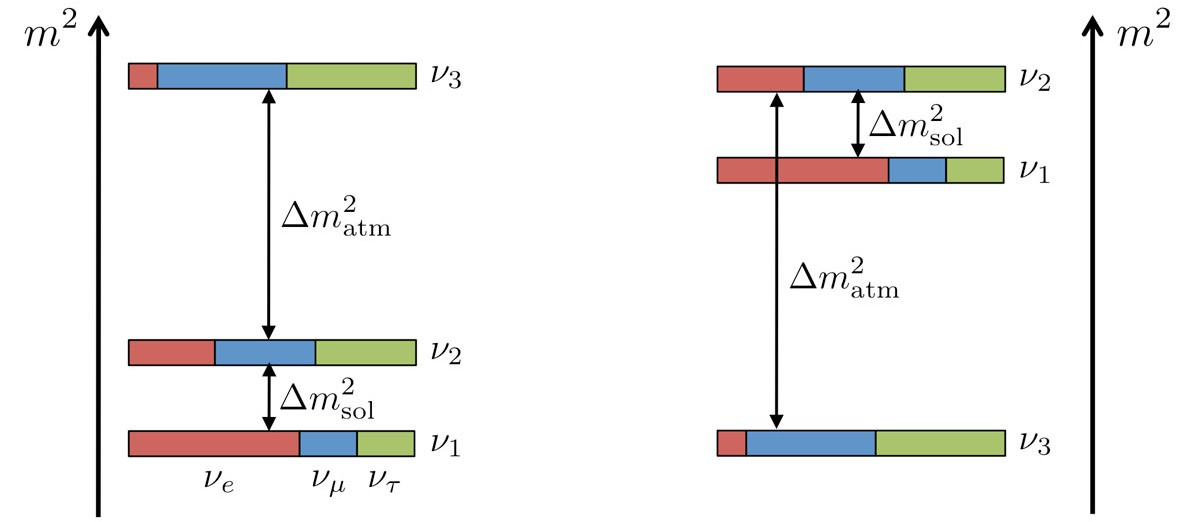
\includegraphics[width = 0.7\textwidth]{figures/mass-hierarchy.jpg}
    \caption{Representation of the two possible mass orderings: normal ordering on the left and inverted ordering on the right.
    The Figure specifies that $\Delta m^2_{21}$ is obtained via solar neutrinos measurements while $\Delta m^2_{32}$ 
    is given by atmospheric neutrinos experiments. Different colours refer to different neutrino flavours: red for the electron flavour, 
    blue for the muon one and green for the tau, respectively. Figure taken from \cite{fermilab-mass-ordering}.}
    \label{fig:mass-ordering}
\end{figure}


\subsection{The Seesaw mechanism}
\label{subsec:seesaw}
Experimental studies confirm that neutrinos do have masses, therefore there must be a corresponding mass term in the Lagrangian. 
Said term can be introduced in the same way as for the up-type quarks\footnote{Recalling the correspondence $u \rightarrow \nu$ and $d \rightarrow \ell$ in the SU(2)$_\text{L}$ doublets.}, using the conjugate Higgs field, yielding a Dirac mass term after the \ac{SSB} as expressed in Eq.~\ref{eq:neutrinos-dirac-masses}
\begin{equation}
    \label{eq:neutrinos-dirac-masses}
    \mathcal{L}_{D} = - m_D (\overline{\nu}_\text{R}\nu_\text{L} + \overline{\nu}_\text{L}\nu_\text{R}) = -\frac{1}{2}m_D (\overline{\nu_\text{L}}\nu_\text{R} + \overline{\nu_\text{R}^c}\nu_\text{L}^c) + \text{h.c.}
\end{equation}
where in the second part we used the equivalence $\overline{\nu_\text{L}}\nu_\text{R} \longleftrightarrow \overline{\nu_\text{R}^c}\nu_\text{L}^c $.
It is clear that if this is the origin of neutrino masses, then \ac{RH}\footnote{Unless otherwise specified, right and left refer to chiral states.}
neutrinos---and \ac{LH} antineutrinos as well---must exist. However, neutrino masses are much smaller than those of other fermions, either the charged leptons or the quarks for which masses arise in the Higgs mechanism, suggesting that there might be a different phenomenon which generates neutrino masses.

Seeing that \ac{RH} neutrinos and \ac{LH} antineutrinos transform as singlets under the \ac{SM} gauge group, any additional term formed by these fields can be added to the \ac{SM} Lagrangian without breaking its gauge invariance.

While \ac{RH} neutrinos appear as such in the new Lagrangian term, \ac{LH} antineutrinos are defined as the \ac{CP} conjugate fields of \ac{RH} neutrinos as written in Eq.~\ref{eq:CPconjugation-righHanded}
\begin{equation}
    \label{eq:CPconjugation-righHanded}
    \psi^c = \hat{C}\hat{P}\psi = i\gamma^2\gamma^0\psi^*.
\end{equation} 
Therefore in the Majorana mass term of Eq.~\ref{eq:neutrinos-majorana-masses}, \ac{LH} antineutrinos are written as $\nu_\text{R}^c$ yielding
\begin{equation}
    \label{eq:neutrinos-majorana-masses}
    \mathcal{L}_M = -\frac{1}{2} M \left( \overline{\nu_\text{R}^c} \nu_\text{R} + \overline{\nu_\text{R}} \nu_\text{R}^c \right).
\end{equation}
 

This term clearly respects the local gauge invariance of the \ac{SM}, and consequently it can be added to the \ac{SM} Lagrangian. 
It is now crucial to notice that the Majorana mass term provides a direct coupling between a particle and an antiparticle. 
Thus the corresponding Majorana mass term for the electron would allow $e^+ \leftrightarrow e^-$ transitions, violating charge conservation. 
This problem does not exist for the neutrinos. Nevertheless, seeing that neutrinos are neutral, it is possible that they are their own 
antiparticles, in which case they are referred to as \textit{Majorana neutrinos} and not as \textit{Dirac neutrinos}.

Finally, we can write the general mass Lagrangian for neutrinos including both Eqs.~\ref{eq:neutrinos-dirac-masses} 
and~\ref{eq:neutrinos-majorana-masses}, obtaining Eq.~\ref{eq:neutrinos-diracANDmajorana-masses}.
\begin{equation}
    \label{eq:neutrinos-diracANDmajorana-masses}
    \mathcal{L}_{DM} = -\frac{1}{2} \left[ m_D \overline{\nu_\text{L}}\nu_\text{R} + m_D \overline{\nu_\text{R}^c}\nu_\text{L}^c + M \overline{\nu_\text{R}^c}\nu_\text{R} \right] + \text{h.c.}
\end{equation}
The two different couplings can be represented using Feynman diagrams as depicted in Figure~\ref{fig:feynman-massCouplings}.
\begin{figure}[H]
    \centering
    \begin{tikzpicture}[
    thick,
    % Stile per i fermioni (linea continua con freccia a metà)
    fermion/.style={draw=black, postaction={decorate},
        decoration={markings, mark=at position 0.55 with {\arrow{latex}}}},
    % Stile per il campo scalare (linea tratteggiata)
    scalar/.style={draw=black, dashed},
    % Stile per la X
    cross/.style={cross out, draw=black, thick, minimum size=8pt, inner sep=0pt},
    % Stile per il vertice puntiforme
    dot/.style={circle, fill=black, minimum size=4pt, inner sep=0pt}
]

% ---------------- DIAGRAMMA DI DIRAC (Sinistra) ----------------
\coordinate (D) at (0,0);

% Linee entrante e uscente
\draw[fermion] (-1.5, 1.5) node[left] {$\nu_L$} -- (D);
\draw[fermion] (D) -- (1.5, 1.5) node[right] {$\nu_R$};

% Linea tratteggiata (Higgs) con la X finale
\draw[scalar] (D) -- (0, -1.5);
\node[cross] at (0, -1.5) {};

% Vertice centrale con pallino e label
\node[dot, label=right:{$m_D$}] at (D) {};


% ---------------- DIAGRAMMA DI MAJORANA (Destra) ----------------
\coordinate (M) at (6, 0.5); % Spostato a destra e leggermente in alto per allineamento visivo

% Linee (entrambe puntano verso il centro)
\draw[fermion] (4, 0.5) node[left] {$\nu_R$} -- (M);
\draw[fermion] (8, 0.5) node[right] {$\overline{\nu}_L$} -- (M);

% Vertice centrale con la X e label
\node[cross, label=above:{$M$}] at (M) {};

\end{tikzpicture}
    \caption{Feynman diagrams of the two possible mass couplings. On the left the Dirac coupling, associated with $m_D$. On the right the Majorana coupling, associated with $M$.}
    \label{fig:feynman-massCouplings}
\end{figure}

Eq.~\ref{eq:neutrinos-diracANDmajorana-masses} can be equivalently rewritten as Eq.~\ref{eq:neutrinos-diracANDmajorana-masses-matrix}
\begin{equation}
    \label{eq:neutrinos-diracANDmajorana-masses-matrix}
    \mathcal{L}_{DM} = -\frac{1}{2} \left( \overline{\nu_\text{L}} \quad \overline{\nu_\text{R}^c} \right) \underbrace{\begin{pmatrix} 0 & m_D \\ m_D & M \end{pmatrix}}_{\mathbf{M}} \begin{pmatrix} \nu_\text{L}^c \\ \nu_\text{R} \end{pmatrix} + \text{h.c.}
\end{equation}

where we identified the mass matrix $\mathbf{M}$, which can be diagonalised in order to define the physical states. 
The characteristic equation $\det(\mathbf{M} - \lambda \mathbb{1}) = 0$ yields $\lambda^2 - M\lambda - m_D^2 = 0$, 
from which one gets the masses of the physical neutrinos 
\begin{equation*}
    m_{\pm} = \lambda_{\pm} = \frac{M \pm \sqrt{M^2 + 4m_D^2}}{2} = \frac{M \pm M\sqrt{1 + 4m_D^2/M^2}}{2}.
\end{equation*}
Furthermore, taking the Majorana mass $M$ much greater than the Dirac mass $m_D$, 
i.e. $M \gg m_D$\footnote{The Dirac mass is assumed to be of the same order of the mass of the other fermions ($\mathcal{O}(1~\text{GeV})$), 
while the Majorana mass term is thought to be very large ($\mathcal{O}(10^{11}~\text{GeV})$) in order to get $m_\nu \sim 0.01$~eV.}, 
the two possible masses reduce to 
\begin{equation*}
    m_{\pm} \approx \frac{1}{2}M \pm \frac{1}{2}\left( M + \frac{2m_D^2}{M} \right)
\end{equation*}
giving a light neutrino state ($\nu$) and a heavy neutrino state ($N$) with the masses reported in Eq.~\ref{eq:final-nu-masses}
\begin{equation}
    \label{eq:final-nu-masses}
    |m_{\nu}| \approx \frac{m_D^2}{M} \quad \text{and} \quad m_N \approx M.
\end{equation} 
Therefore, if we go back to Eq.~\ref{eq:neutrinos-diracANDmajorana-masses-matrix}, we can rewrite $\nu$ and $N$ as a function of
$\nu_\text{L}$, $\nu_\text{L}^c$, $\nu_\text{R}$ and $\nu_\text{R}^c$ as shown in Eq.~\ref{eq:neutrinos-revisited}
\begin{equation}
    \label{eq:neutrinos-revisited}
    \nu = \cos\theta (\nu_\text{L} + \nu_\text{L}^c) - \sin\theta (\nu_\text{R} + \nu_\text{R}^c) \quad \text{and} \quad N = \cos\theta (\nu_\text{R} + \nu_\text{R}^c) + \sin\theta (\nu_\text{L} + \nu_\text{L}^c)
\end{equation}
where the mixing angle $\theta$ is determined by the ratio of the Dirac and Majorana masses, with $\theta = \frac{m_D}{M}$. 
Since the Majorana mass scale $M$ is assumed to be enormous compared to the Dirac mass, this ratio is extremely small. 
Consequently, $\theta$ tends to zero and this allows us to apply the small-angle approximations for the trigonometric functions such that
$\tan\theta \sim \theta \sim \frac{m_D}{M}~$ and consequently one gets $~\cos\theta \sim 1~$ and $~\sin\theta \sim \theta = \frac{m_D}{M}~$.\\
This consideration yields
\begin{equation*}
    \nu \approx (\nu_\text{L} + \nu_\text{L}^c) - \frac{m_D}{M}(\nu_\text{R} + \nu_\text{R}^c) ~ \text{and} ~ N \approx (\nu_\text{R} + \nu_\text{R}^c) + \frac{m_D}{M}(\nu_\text{L} + \nu_\text{L}^c).
\end{equation*}
It is now evident that the light-neutrino state is almost entirely \ac{LH} while the heavy-neutrino one is almost entirely \ac{RH}. 
Therefore, the latter participates neither in the weak \ac{CC} interactions nor in the weak \ac{NC} interactions of the \ac{SM}.

The process described so far, set against the Higgs mechanism for mass, is known as \textit{seesaw mechanism}.
It is only a hypothesis, but it would be more grounded if neutrinos were shown to be Majorana particles.
Their Majorana nature could be established by observing neutrinoless double $\beta$-decay, which is discussed in Section~\ref{sec:0nubetabeta}.